In recent years, there has been a significant increase in the use of micro aerial vehicles (MAVs) or unmanned aerial vehicles (UAVs), also known as drones, in various industries such as agriculture, real estate, filmography, and delivery services. This is primarily due to their versatility and cost-effectiveness. As a result, there is a growing demand for multi-drone systems that can collaborate and operate in real-world dynamic environments.

However, operating multiple drones in such environments poses several challenges. These challenges include navigating around moving obstacles, coordinating the actions of multiple drones, and adapting to real-time changes in the environment. Traditional motion planning and control algorithms often struggle to handle the complexity and unpredictability of these scenarios.

In order to address these challenges, this paper proposes a solution based on deep reinforcement learning (DRL). DRL is a branch of machine learning that combines deep learning techniques with reinforcement learning to enable agents to learn and make decisions in complex environments. By training the drones using DRL algorithms, they can learn to effectively navigate in dynamic environments and avoid collisions with moving obstacles.

The objective of this paper is to develop a multi-drone motion planning and control system that can operate in real-world dynamic environments. The system will be based on DRL algorithms and will be capable of coordinating the actions of multiple drones while avoiding collisions with obstacles in real-time. The performance of the proposed system will be evaluated through simulations and real-world experiments.

The rest of the paper is organized as follows. In Section II, we provide a literature review of existing research in the field of multi-drone motion planning and control. Section III describes the problem statement and the proposed approach. Section IV presents the experimental setup and the evaluation metrics used. The results and discussions are presented in Section V, followed by the conclusions and future work in Section VI.Traditional planning and control pipelines have been extensively studied in recent decades in the literature for robots' autonomous navigation. Numerous complete systems, incorporating simultaneous localization and mapping (SLAM) and hierarchical planning and control frameworks, have achieved outstanding autonomy. For instance, Zhou et al. (2019) propose a robust and efficient quadrotor motion planning system for fast flight in three-dimensional complex environments. Quan et al. (2023) introduce a distributed motion planning trajectory optimization framework for large-scale quadrotor formation flight in dense environments. Despite the great performance that traditional methods can achieve, they face certain limitations and challenges:

\begin{itemize}
  \item \textbf{Complexity}: The hierarchical planning and control methods consist of numerous layers of modules, each requiring fine-tuning of parameters, thereby increasing the overall complexity of the system.
  \item \textbf{Modeling Limitation}: Traditional methods heavily rely on accurate models of the environment and the system. However, creating precise models, particularly for complex systems like drones, can be a challenging task. Even small discrepancies between the model and reality can result in significant performance degradation.
  \item \textbf{Generalizability}: Many traditional methods are specifically tailored to particular tasks, environments, or robot platforms. Transferring them to new tasks or settings often necessitates substantial modifications.
\end{itemize}

The classical hierarchical motion planning framework's capability is challenged as the complexity and randomness of robot application scenarios increase. Recent advancements in artificial intelligence have resulted in the development of Deep Reinforcement Learning (DRL), a branch of machine learning that trains agents to make sequential decisions through interaction with an environment. DRL has shown promise in addressing complex problems in robotics due to its ability to learn from large amounts of data and adapt to changes in real-time (Lee et al., 2020; Hwangbo et al., 2017; Gu et al., 2017). DRL-based motion planning and control offer insights to overcome the challenges faced by traditional methods:

\begin{itemize}
  \item \textbf{Unified framework}: DRL enables unified end-to-end training and inference, where both planning and control can be learned jointly, potentially leading to more cohesive and optimal solutions.
  \item \textbf{Scalability with multiple agents}: DRL can be extended to multi-agent scenarios using techniques like multi-agent reinforcement learning, allowing for cooperative or competitive behaviors among agents.
  \item \textbf{Data-driven model}: In contrast to model-based methods that require precise system models, DRL can learn planning and control policies directly from interaction data, potentially avoiding modeling inaccuracies.
  \item \textbf{Generalization}: Since many DRL methods are model-free, the training can be generalized to different robot platforms and even other tasks by changing the reward functions defined in DRL algorithms.
\end{itemize}

Traditional motion planning and control methods have long provided reliable solutions in robotics. However, as tasks become increasingly complex, such as navigating in dynamic and stochastic environments, their limitations become evident. In this report, we propose utilizing the adaptability of DRL to address these limitations. Our objective is to guide a quadrotor team through a combination of static and dynamic gates, aiming for maximum scores in minimal time. This task will showcase the potential of DRL in advanced robotic navigation challenges.

\section{Related Work}
In this section, we will explore both traditional and RL-based methods for planning and control in the literature, with a particular focus on aerial systems such as drones or quadrotors. Traditional planning and control frameworks are typically decoupled.The path-planning module serves as a guide system for the low-level controller that drives the robot's movement. This module is responsible for generating a geometrically collision-free and possibly kinodynamically feasible trajectory (or motion setpoints) for the low-level controller. The low-level control module can then use these motion setpoints to control the robot's actuators for movement.

Recent reinforcement learning (RL)-based methods attempt to combine these two modules into a coupled system through repeated learning. The robots learn to navigate themselves through trials and learning from their environments. These trials are mostly conducted in simulations, which require high-fidelity physics engines. By utilizing specific (deep) RL training methods, the trained models (e.g., neural networks) can be deployed on real robots for autonomous navigation in various static or dynamic environments.

\subsection{Configuration Space and Map Representation}
The configuration space (C-Space) encompasses all possible transformations for the robots. For a robot with n degrees of freedom, the set of transformations, which forms a manifold with a dimension of n, is defined as the configuration space for that robot, denoted as \robotConfig \cite{quan2020survey}. For instance, the C-Space for a 2D rigid body is $SE(2)$, and for a 3D rigid body, it is $SE(3)$.

The obstacle region \robotConfig_{\text{obs}}\subseteq \robotConfig corresponds to the transformations that result in collisions between the robot and the obstacles. Conversely, the free space is defined as \robotConfig_{\text{free}} = \robotConfig \backslash \robotConfig_{\text{obs}}. Therefore, the motion planning problem can be formulated as finding a path \tau : [0,1]\rightarrow \robotConfig_{\text{free}}, such that \tau(0) = q_{\text{start}} \in \robotConfig_{\text{free}} and \tau(1) = q_{\text{goal}} \in \robotConfig_{\text{free}} represent the start and goal transformations, respectively.

Although mapping techniques are typically associated with simultaneous localization and mapping (SLAM) problems, mapping with a known robot pose is also crucial. Many motion planning algorithms assume a given map. One prevalent map representation is the occupancy grid map \cite{elfes2013occupancy}, in which space is divided into cells (2D or 3D) that store the probabilistic estimate of their occupancy states.

Various data structures can efficiently represent the space. The K-Dimensional Tree (K-D Tree), an efficient data structure for organizing multi-dimensional point data \cite{bentley1975multidimensional}, allows for rapid search of nearest neighbors. The Incremental K-D Tree (ikd-tree) \cite{cai2021ikd} enables incremental updates to the K-D tree with new points.

Octomap \cite{wurm2010octomap}, based on octrees and using probabilistic occupancy estimation, proposes a compact data structure for map representation. Another approach for volumetric representation is based on signed distance fields (SDFs), introduced in computer graphics literature \cite{curless1996volumetric}. In recent robotic applications, truncated signed distance fields (TSDFs) \cite{lin2018autonomous} are used to reconstruct the surfaces around the MAV (micro aerial vehicle). Euclidean signed distance fields (ESDFs) \cite{oleynikova2017voxblox,han2019fiesta} are used to incrementally update the voxel map with distance and gradient information, providing more convenient gradient-based trajectory optimization.

\subsection{Traditional Planning and Control Methods}\begin{figure}[h]
\center
\begin{adjustbox}{width=.5\textwidth}

\tikzset{every picture/.style={line width=0.75pt}} %set default line width to 0.75pt        

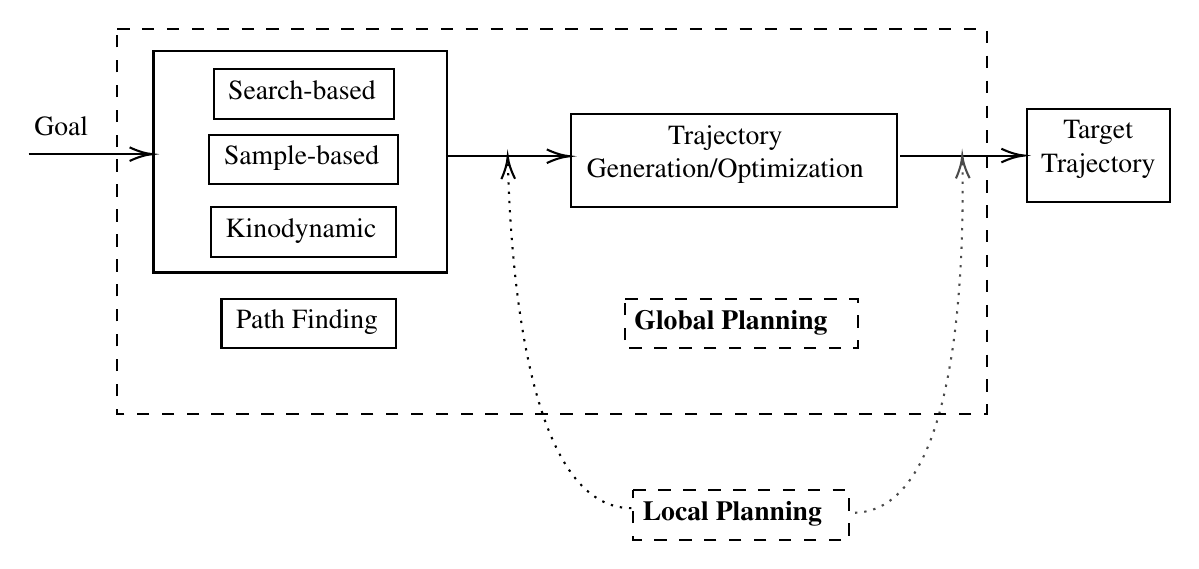
\begin{tikzpicture}[x=0.75pt,y=0.75pt,yscale=-1,xscale=1]
%uncomment if require: \path (0,267); %set diagram left start at 0, and has height of 267

%Shape: Rectangle [id:dp575866165243341] 
\draw   (89.56,19.67) -- (230.89,19.67) -- (230.89,126.44) -- (89.56,126.44) -- cycle ;
%Straight Lines [id:da8414235785777104] 
\draw    (230.44,70.44) -- (288,70.44) ;
\draw [shift={(290,70.44)}, rotate = 180] [color={rgb, 255:red, 0; green, 0; blue, 0 }  ][line width=0.75]    (10.93,-3.29) .. controls (6.95,-1.4) and (3.31,-0.3) .. (0,0) .. controls (3.31,0.3) and (6.95,1.4) .. (10.93,3.29)   ;
%Straight Lines [id:da08815651015896142] 
\draw    (29.44,69.44) -- (87,69.44) ;
\draw [shift={(89,69.44)}, rotate = 180] [color={rgb, 255:red, 0; green, 0; blue, 0 }  ][line width=0.75]    (10.93,-3.29) .. controls (6.95,-1.4) and (3.31,-0.3) .. (0,0) .. controls (3.31,0.3) and (6.95,1.4) .. (10.93,3.29)   ;
%Straight Lines [id:da22108099082080424] 
\draw    (449.44,70.11) -- (507,70.11) ;
\draw [shift={(509,70.11)}, rotate = 180] [color={rgb, 255:red, 0; green, 0; blue, 0 }  ][line width=0.75]    (10.93,-3.29) .. controls (6.95,-1.4) and (3.31,-0.3) .. (0,0) .. controls (3.31,0.3) and (6.95,1.4) .. (10.93,3.29)   ;
%Curve Lines [id:da017803972324741846] 
\draw [color={rgb, 255:red, 0; green, 0; blue, 0 }  ,draw opacity=1 ] [dash pattern={on 0.84pt off 2.51pt}]  (319.78,240) .. controls (270.94,240) and (261.74,130.66) .. (260.26,72.2) ;
\draw [shift={(260.22,70.44)}, rotate = 88.68] [color={rgb, 255:red, 0; green, 0; blue, 0 }  ,draw opacity=1 ][line width=0.75]    (10.93,-3.29) .. controls (6.95,-1.4) and (3.31,-0.3) .. (0,0) .. controls (3.31,0.3) and (6.95,1.4) .. (10.93,3.29)   ;
%Curve Lines [id:da912860022154641] 
\draw [color={rgb, 255:red, 74; green, 74; blue, 74 }  ,draw opacity=1 ] [dash pattern={on 0.84pt off 2.51pt}]  (427.56,242.22) .. controls (475.74,240.9) and (480.46,130.36) .. (479.26,71.87) ;
\draw [shift={(479.22,70.11)}, rotate = 88.68] [color={rgb, 255:red, 74; green, 74; blue, 74 }  ,draw opacity=1 ][line width=0.75]    (10.93,-3.29) .. controls (6.95,-1.4) and (3.31,-0.3) .. (0,0) .. controls (3.31,0.3) and (6.95,1.4) .. (10.93,3.29)   ;
%Shape: Rectangle [id:dp5818665047698117] 
\draw  [dash pattern={on 4.5pt off 4.5pt}] (72,9) -- (491,9) -- (491,194.5) -- (72,194.5) -- cycle ;

% Text Node
\draw    (122.33,139) -- (206.33,139) -- (206.33,163) -- (122.33,163) -- cycle  ;
\draw (125.33,143) node [anchor=north west][inner sep=0.75pt]   [align=left] {\begin{minipage}[lt]{55.15pt}\setlength\topsep{0pt}
\begin{center}
{\fontfamily{ptm}\selectfont Path Finding}
\end{center}

\end{minipage}};
% Text Node
\draw    (118.5,28.5) -- (205.5,28.5) -- (205.5,52.5) -- (118.5,52.5) -- cycle  ;
\draw (121.5,32.5) node [anchor=north west][inner sep=0.75pt]   [align=left] {\begin{minipage}[lt]{57.1pt}\setlength\topsep{0pt}
\begin{center}
{\fontfamily{ptm}\selectfont Search-based}
\end{center}

\end{minipage}};
% Text Node
\draw    (116.5,60) -- (207.5,60) -- (207.5,84) -- (116.5,84) -- cycle  ;
\draw (119.5,64) node [anchor=north west][inner sep=0.75pt]   [align=left] {\begin{minipage}[lt]{59.94pt}\setlength\topsep{0pt}
\begin{center}
{\fontfamily{ptm}\selectfont Sample-based}
\end{center}

\end{minipage}};
% Text Node
\draw    (117.33,95) -- (206.33,95) -- (206.33,119) -- (117.33,119) -- cycle  ;
\draw (120.33,99) node [anchor=north west][inner sep=0.75pt]   [align=left] {\begin{minipage}[lt]{58.25pt}\setlength\topsep{0pt}
\begin{center}
{\fontfamily{ptm}\selectfont Kinodynamic}
\end{center}

\end{minipage}};
% Text Node
\draw    (290.78,50) -- (447.78,50) -- (447.78,95) -- (290.78,95) -- cycle  ;
\draw (293.78,54) node [anchor=north west][inner sep=0.75pt]   [align=left] {\begin{minipage}[lt]{104.69pt}\setlength\topsep{0pt}
\begin{center}
{\fontfamily{ptm}\selectfont Trajectory }\\{\fontfamily{ptm}\selectfont Generation/Optimization}
\end{center}

\end{minipage}};
% Text Node
\draw (30.67,49.67) node [anchor=north west][inner sep=0.75pt]   [align=left] {{\fontfamily{ptm}\selectfont Goal}};
% Text Node
\draw    (510.33,47.67) -- (579.33,47.67) -- (579.33,92.67) -- (510.33,92.67) -- cycle  ;
\draw (513.33,51.67) node [anchor=north west][inner sep=0.75pt]   [align=left] {\begin{minipage}[lt]{44.84pt}\setlength\topsep{0pt}
\begin{center}
{\fontfamily{ptm}\selectfont Target }\\{\fontfamily{ptm}\selectfont Trajectory}
\end{center}

\end{minipage}};
% Text Node
\draw  [dash pattern={on 4.5pt off 4.5pt}]  (320.8,231.22) -- (424.8,231.22) -- (424.8,255.22) -- (320.8,255.22) -- cycle  ;
\draw (323.8,235.22) node [anchor=north west][inner sep=0.75pt]   [align=left] {{\fontfamily{ptm}\selectfont \textbf{Local Planning}}};
% Text Node
\draw  [dash pattern={on 4.5pt off 4.5pt}]  (316.8,139) -- (428.8,139) -- (428.8,163) -- (316.8,163) -- cycle  ;
\draw (319.8,143) node [anchor=north west][inner sep=0.75pt]   [align=left] {{\fontfamily{ptm}\selectfont \textbf{Global Planning}}};


\end{tikzpicture}
\end{adjustbox}
\caption{Hierarchical planning pipeline: The path-finding module 
finds a geometric collision-free path, and then trajectory
optimization module generates a state-admissable kinodynamic
feasible trajectory. Local planning methods can be 
incorporated in different stages.}
\label{fig:concept}
\end{figure}


In general, path-planning algorithms for robot navigation can be divided into two major categories: global and local methods \cite{Lavalle-2006}. Global methods focus on finding collision-free paths from the current robot position to a global goal position, mostly in static scenes. On the other hand, local methods tend to reactively avoid both static and dynamic obstacles. It should be noted that there is no strict line between global and local planning methods, as it can also be argued that with high-frequency global re-planning, local path planning can be avoided \cite{fraichard-2020}.

In order to generate smooth trajectories for robots to follow based on the discrete planned waypoints, a trajectory optimization module is usually added in the entire pipeline. The path-finding module is commonly referred to as the frontend, while the trajectory optimization module is called the backend. A typical traditional planning pipeline is illustrated in Figure \ref{fig:concept}.

\subsubsection{Path finding (frontend)}
In the path-finding stage of global planning, the methods can be categorized into three major directions: search-based, sample-based, and kinodynamic methods.

\textbf{Search-based} algorithms, such as Depth-First Search (DFS) \cite{cormen-2009}, Breadth-First Search (BFS) \cite{cormen-2009}, Dijkstra's Algorithm \cite{dijkstra-1959}, and the A* algorithm \cite{hart-1968}, use graph-search methods, possibly with pre-defined heuristics, to find geometrically feasible paths on given grid maps. These methods assume that the map is given, which can be challenging to obtain in certain situations. While these search-based methods can perform well, they may have longer search times as the space scales.

\textbf{Sample-based} methods, such as Rapidly Exploring Random Trees (RRT), Probabilistic Roadmaps (PRM), and their variants (e.g., RRT* and PRM*), use sampling in the configuration space (C-Space) to create collision-free paths \cite{lavalle-1998,kavraki-1996,karaman-2011}. The general form of the RRT algorithm is shown in Algorithm \ref{alg:rrt}. However, the tree nodes in these methods need to cover the entire C-Space, which may lead to heavy computational loads, especially when the space is large.

Both search-based and sample-based methods can generate geometrically collision-free paths but these paths may be jerky or violate the underlying robots' dynamics. For instance, most ground vehicles are not holonomic, meaning they cannot move freely in all directions in 2D space. Their motions are governed by mechanical and motion constraints, such as velocities and accelerations \cite{lavalle-2006}. To adhere to both the kinematic and dynamic constraints specific to robot platforms and reduce the load on the backend optimization part, kinodynamic methods are introduced in the literature \cite{donald-1993}. 

The term \textbf{kinodynamic} motion planning was first proposed by Donald \textit{et al.} \cite{donald-1993} in the literature. The authors presented the first provably good approximation algorithm for motion planning of a point-mass model in 2D and 3D environments with polyhedral obstacles. The state-lattice method \cite{pivtoraiko-2011} is also used for kinodynamic motion planning, where the boundary value problem (BVP) needs to be solved to obtain the corresponding control inputs for the sampled states. In \cite{zhou-2019}, the authors propose a method that samples in the control space to generate possible motion primitives and then searches and selects kinodynamically feasible paths. Webb and Berg \cite{webb-2013} generalize the kinodynamic RRT* method, extending the earlier work on RRT* \cite{karaman-2011}, to guarantee asymptotic optimality for any system with controllable linear dynamics in state spaces of any dimension. Additionally, hybrid A* (or hybrid-state A*) algorithms are proposed in \cite{dolgov-2008,dolgov-2009,dolgov-2010} as extensions of the original A* algorithm for kinodynamic graph searching.Other less common methods, such as model predictive control (MPC) added with obstacle constraints or additional environment-related terms (Park et al., 2009; Ji et al., 2016), can also be used to generate collision-free paths. These methods are based on quadratic programming (QP) optimization. However, MPC-related methods require a tradeoff between the length of the time horizon, computational loads, and optimality. A short time horizon often leads to sub-optimal solutions.

\subsubsection{Trajectory Generation and Optimization (Backend)}
Most path-finding algorithms only generate geometrically feasible paths without any time information. The goal of trajectory generation and optimization is to provide both spatial and temporal profiles based on the found paths (Quan et al., 2020). Essentially, the trajectory is a geometric path parameterized in time, guaranteeing kinodynamic feasibility and smoothness. It is usually optimized to minimize the total "energy" spent along the path while satisfying the kinodynamic constraints of the robots.

Mellinger and Kumar (2011) propose a minimum snap trajectory generation method based on the differential flat property of quadrotor or multirotor systems. This method utilizes quadratic programming (QP) optimization with hard constraints for flight corridors to generate optimal trajectories.

Interpolating curves are one of the prevalent methods in the literature (Dong et al., 2023). Zhou et al. (2019) propose a trajectory optimization method based on the convex hull property of B-splines and provide a time adjustment method for it. Wang et al. (2022) propose a minimum-control (MINCO) trajectory family based on multi-degree polynomials, which can be optimized with user-defined state-input constraints for multi-copter motion planning.

Gradient-based methods, such as CHOMP (Ratliff et al., 2009) and EGO-Planner (Zhou et al., 2020), are also popular for trajectory optimization.\subsubsection{Local Methods}
While global methods often perform well in static environments, they tend to struggle in dynamic environments. To address this issue, local path-planning methods can be employed. One early method is the artificial potential field (APF) \cite{warren1989global}. APF formulates the potentials along a given path as both inside and outside potentials, and guides the path from regions of high potential to low potential by seeking the lowest potential value. For waypoints on the path that pass through or inside an obstacle, the potential is defined as:

\begin{equation}
\label{eq:APF_in}
U_{\text{in}} = 
U_{\text{max}}(1 - \frac{R_{\text{in}}}{R_{\text{max}}}) + 
U_{\text{offset}}
\end{equation}

Here, $U_{\text{max}}$ represents the maximum potential, $R_{\text{in}}$ is the distance to the centroid of the obstacle, $R_{\text{max}}$ is the maximum radius of the obstacle, and $U_{\text{offset}}$ is an additional potential penalty. The outside potential is formulated as:

\begin{equation}
\label{eq:APF_out}
U_{\text{out}} = 
\frac{1}{2}U_{\text{offset}}(1+ \frac{1}{1+R_\text{out}})
\end{equation}

$R_{\text{out}}$ denotes the distance outside the obstacle. APF has been applied to quadrotor path-planning \cite{chen2016uav}. However, when dealing with multiple obstacles, APF may suffer from the issue of local minima \cite{koren1991potential}. Another method for dynamic obstacle avoidance is the dynamic window approach (DWA) \cite{seder2007dynamic}. DWA takes into account the robot's kinodynamic feasibility and samples motion primitives in the velocity space to avoid collisions. The concept of velocity obstacle (VO) was proposed and generalized by Van Den Berg \cite{van2011reciprocal,van2011reciprocal2,bareiss2013reciprocal}. Methods based on reciprocal VO can be used for robot motion planning. However, the smoothness of the generated paths cannot be guaranteed. Another approach to local motion planning is dynamical system modulation (DSM) \cite{khansari2012dynamical,huber2022fast,huber2023avoidance}. DSM directly modifies the first-order linear system, based on the robot's point-mass model, by adding a linear transformation obtained from the environment to the initial velocity of the robot. However, these algorithms are limited to star-shaped obstacles, and the performance of DSM on agile robots such as quadrotors remains uncertain.

\subsubsection{Control}
The control module is primarily responsible for trajectory tracking (TT) in planning and control. In addition to the low-level controllers that track the setpoints of torques, angular velocities, or accelerations of the actuators, the controllers used in the TT phase focus on designing controllers based on system equations to enable robots to asymptotically track a given reference trajectory. For instance, \cite{majd2019stable} proposes the use of input-output linearization technique to optimize the tracking error for car-like robot trajectory tracking. Model predictive control (MPC) or receding horizon control (RHC) is another widely used method for TT through optimization. \cite{kunhe2005mobile} employs nonlinear MPC to control wheeled robots for TT. \cite{romero2022model,ji2021cmpcc} propose model predictive contouring control (MPCC) by incorporating the time profile into the controller design to minimize traversal time while tracking the reference trajectory. Thanks to the versatility of the MPC framework, the model can be reformulated to suit different requirements. In \cite{zhang2023coni}, the authors propose cooperative non-inertial frame based model predictive control (CoNi-MPC), which directly formulates the quadrotor model in the non-inertial frame of a target and controls the quadrotor to track trajectories predefined in the target's frame.\subsection{Deep Reinforcement Learning (DRL)-based Planning and Control}
Deep Reinforcement Learning (DRL), which combines deep learning and reinforcement learning (RL), has become increasingly popular in the field of motion planning and control. Its adaptability, ability to learn from raw data, and scalability have made it an attractive choice for researchers \cite{mnih2015human}. For instance, Mnih et al. introduced the deep Q network (DQN), a DRL algorithm capable of achieving human-level performance in various video games. This breakthrough has established a precedent for applying DQN in motion planning and control for robots. Additionally, Lillicrap et al. went on to expand the capabilities of DQN by proposing the deep deterministic policy gradient (DDPG) algorithm. This algorithm facilitates learning policies in continuous action spaces, a necessary feature for most real-world control tasks \cite{lillicrap2015continuous}.

In the context of aerial vehicles, Zhang et al. integrated Model Predictive Control (MPC) with DRL. They demonstrated the combination through guided policy search with an MPC controller in simulation. Their work employed a policy that maps raw sensor data to rotor velocities to achieve obstacle avoidance \cite{zhang2016learning}. Moreover, Kahn et al. proposed a DRL methodology that excelled in navigation tasks using raw monocular camera images \cite{kahn2018self}.

The application of DRL in drone racing and agile flight dynamics has received significant attention in recent studies \cite{loquercio2019deep, song2021autonomous, song2022policy, penicka2022learning, song2023reaching}. These studies highlight the effectiveness of DRL in motion planning and control, particularly in addressing the demands of high-speed agile navigation for quadrotors.

\subsection{Multi-robot Planning and Control}

\section{Problem Formulation}

\subsection{Quadrotor Dynamics}

\subsection{Task Formulation}

\bibliographystyle{IEEEtran}
\bibliography{report}

\end{document}